\documentclass[11pt,a4paper]{article}

\usepackage[utf8]{inputenc}
\usepackage[T1]{fontenc}
\usepackage[spanish,es-tabla]{babel}
\usepackage{geometry}
\geometry{left=2.3cm,right=2.3cm,top=2.5cm,bottom=2.5cm}

\usepackage{amsmath,amssymb,amsthm}
\usepackage{booktabs}
\usepackage{graphicx}
\usepackage{float}
\usepackage{caption}
\usepackage{subcaption}
\usepackage{xcolor}
\usepackage{hyperref}
\usepackage{listings}
\usepackage{enumitem}
\usepackage{fancyhdr}
\usepackage{array}
\usepackage{longtable}

\definecolor{uchileblue}{RGB}{0,56,118}
\definecolor{darkred}{RGB}{180,30,30}
\definecolor{darkgreen}{RGB}{20,120,60}
\definecolor{codebg}{RGB}{247,248,250}

\hypersetup{
    colorlinks=true,
    linkcolor=uchileblue,
    citecolor=uchileblue,
    urlcolor=uchileblue,
    pdftitle={Informe Final Proyecto CC5212 - Grupo 13 - Ranking Financiero vs Estructural en ChileCompra 2025},
    pdfauthor={Grupo 13 - CC5212 Procesamiento Masivo de Datos}
}

\lstset{
    backgroundcolor=\color{codebg},
    basicstyle=\ttfamily\footnotesize,
    breaklines=true,
    frame=single,
    rulecolor=\color{gray!40},
    numbers=left,
    numberstyle=\tiny\color{gray},
    keywordstyle=\color{uchileblue}\bfseries,
    commentstyle=\color{darkgreen}\itshape,
    stringstyle=\color{darkred},
    showstringspaces=false,
    tabsize=2,
    literate={á}{{\'a}}1 {é}{{\'e}}1 {í}{{\'\i}}1 {ó}{{\'o}}1 {ú}{{\'u}}1 {ñ}{{\~n}}1 {Ñ}{{\~N}}1
}

\newtheorem{proposition}{Proposición}

\pagestyle{fancy}
\fancyhf{}
\lhead{\small \textbf{CC5212 --- Procesamiento Masivo de Datos}}
\rhead{\small \textbf{Grupo 13 --- Primavera 2026}}
\cfoot{\thepage}

\begin{document}

% ============================================================================
% PORTADA / ENCABEZADO ACADÉMICO
% ============================================================================
\begin{titlepage}
    \centering
    \vspace*{1.0cm}
    {\scshape\Large Universidad de Chile \par}
    {\scshape\large Facultad de Ciencias Físicas y Matemáticas \par}
    {\scshape\large Departamento de Ciencias de la Computación \par}
    \vspace{1.2cm}
    \rule{\linewidth}{0.6mm} \\[0.4cm]
    {\huge \bfseries \color{uchileblue} Detección de Perfiles Estructurales y Financieros en las Compras Públicas de Chile (2025): \\[0.25cm]
    \Large Un Enfoque Híbrido de Agregación Masiva y Centralidad Ponderada en Grafos Bipartitos \par}
    \vspace{0.2cm}
    \rule{\linewidth}{0.6mm} \\[1.2cm]

    {\Large \textbf{Informe Final del Proyecto de Curso} \par}
    \vspace{0.3cm}
    {\large \textbf{CC5212-1: Procesamiento Masivo de Datos} \par}
    \vspace{1.2cm}

    \begin{tabular}{ll}
        \textbf{Grupo:} & Grupo 13 \\
        \textbf{Profesor:} & Alberto Moya L. \\
        \textbf{Semestre:} & Primavera 2026 \\
        \textbf{Fecha:} & Noviembre de 2026
    \end{tabular}

    \vfill
    \begin{abstract}
    \noindent
    El presente informe aborda el procesamiento masivo y modelado estructural de la totalidad de las Órdenes de Compra (OC) emitidas a través del portal MercadoPúblico (ChileCompra) durante los 12 meses del año 2025. A partir de un repositorio bruto de \textbf{5.141.233 registros a nivel de línea de ítem} ($\sim 8,7\text{ GB}$ en 12 archivos CSV mensuales con 79 atributos), diseñamos e implementamos una arquitectura completa ejecutada localmente en multiproceso y compatible con Apache Pig y Apache Giraph. Primero, realizamos una auditoría forense de calidad de datos que colapsa la estructura maestro-detalle a \textbf{1.856.075 órdenes únicas} (\textbf{1.853.435 órdenes válidas}) y corrige distorsiones severas de digitación monetaria (45 órdenes con falsa moneda extranjera/reajustable en UF/UTM/USD cuyos ítems estaban en pesos y 21 órdenes atípicas irrecuperables $\ge \$10^{10}\text{ CLP}$), reduciendo el gasto aparente desde $\$45,80\text{ billones}$ hasta el valor real de \textbf{$\$18,18\text{ billones de CLP}$} ($-60,3\%$). Segundo, modelamos el ecosistema como un grafo bipartito $G=(O \cup P, E)$ compuesto por \textbf{1.165 organismos públicos}, \textbf{75.603 proveedores} y \textbf{476.717 relaciones comerciales únicas}. Demostramos matemática y empíricamente que el modelo de PageRank dirigido simple ($O \to P$) degenera al colapsar los 1.165 organismos a un único valor constante ($c_0 = 1,9539 \times 10^{-6}$) y penalizar a los grandes compradores ($\propto 1/\text{deg}^+(u)$). Para superarlo, implementamos un modelo de \textbf{PageRank Bipartito Bidireccional Ponderado} ($w_{uv} = \ln(1 + M_{uv})$) que permite contrastar el ranking puramente financiero con la centralidad de red, caracterizando empíricamente los dos perfiles propuestos por la cátedra: (1) \textbf{Alto Monto y Bajo PageRank} (adjudicatarios monopsónicos de mega-contratos en JUNAEB y constructoras hospitalarias que caen $>36.000$ puestos en red) y (2) \textbf{Bajo Monto y Alto PageRank} (proveedores hiper-capilares y PYMEs de \textit{Compra Ágil} que abastecen a cerca de 300 organismos públicos situándose en el Top $0,2\%$ estructural del Estado).
    \end{abstract}
    \vfill
\end{titlepage}

\tableofcontents
\newpage

% ============================================================================
% SECCIÓN 1: INTRODUCCIÓN Y MOTIVACIÓN
% ============================================================================
\section{Introducción y Motivación}

El sistema de compras públicas de Chile, administrado por la Dirección ChileCompra a través de la plataforma transaccional \textit{MercadoPúblico}, canaliza anualmente más de dieciocho billones de pesos chilenos en adquisiciones de bienes y servicios indispensables para el funcionamiento del Estado: desde insumos clínicos hospitalarios, raciones de alimentación escolar y obras de infraestructura vial, hasta suministros cotidianos de ferretería, combustible y servicios tecnológicos para municipalidades, universidades y ramas de las Fuerzas Armadas.

Tradicionalmente, el análisis de las contrataciones estatales se ha restringido a consultas de agregación contable (\texttt{GROUP BY} / \texttt{SUM}) orientadas a responder quiénes son los proveedores que adjudican los mayores montos monetarios. Sin embargo, como destacó el profesor Alberto Moya en la retroalimentación del proyecto, \textbf{importancia financiera no equivale a importancia estructural}:
\begin{enumerate}[label=\arabic*.]
    \item Existen empresas que adjudican sumas multimillonarias mediante \textbf{un único contrato masivo} con una sola repartición pública (alta concentración financiera, pero nula transversalidad en el aparato estatal).
    \item En el extremo opuesto, existen proveedores que, sin poseer los contratos más costosos del año, \textbf{abastecen simultáneamente a cientos de los organismos públicos más importantes, transversales o críticos del país}, actuando como verdaderos conectores operativos de la red pública.
\end{enumerate}

El objetivo central de este proyecto es diseñar, ejecutar y validar de extremo a extremo un flujo de procesamiento masivo de datos sobre los 12 meses del año 2025 ($5.141.233$ registros) que combine dos paradigmas complementarios vistos en el curso CC5212:
\begin{itemize}
    \item \textbf{Procesamiento relacional masivo (Apache Pig / Pipeline Multiproceso Local):} Para la limpieza, deduplicación a nivel de orden de compra y cálculo de los rankings financieros, de volumen transaccional, capilaridad institucional, concentración sectorial y desigualdad (Gini/Pareto).
    \item \textbf{Procesamiento paralelo de grafos (Apache Giraph / Modelo Pregel BSP):} Para modelar la red bipartita comprador--proveedor y calcular métricas de centralidad estructural mediante \textbf{PageRank y PageRank Ponderado}, cruzando ambos rankings para identificar y caracterizar rigurosamente los dos perfiles estratégicos de proveedores del Estado.
\end{itemize}

Toda la ejecución analítica que se presenta en este informe fue resuelta íntegramente en nuestro entorno local (procesador AMD Ryzen 5 5600H de 12 hilos lógicos y 14 GB de RAM) mediante algoritmos en \textit{streaming} y multiproceso que emulan de forma matemáticamente exacta las primitivas de Apache Pig y Apache Giraph, contrastando además nuestros resultados punto por punto frente al cuaderno de preparación en Google Colab desarrollado en paralelo por el equipo.

% ============================================================================
% SECCIÓN 2: ARQUITECTURA DE DATOS Y AUDITORÍA FORENSE DE LIMPIEZA
% ============================================================================
\section{Arquitectura de Datos y Auditoría Forense de Limpieza}

\subsection{Estructura Maestro-Detalle Desnormalizada de los 12 Archivos CSV}

Los datos crudos provienen del portal de Descargas Masivas de Datos Abiertos de ChileCompra (\url{https://datos-abiertos.chilecompra.cl/descargas}) y comprenden 12 archivos mensuales (\texttt{2025-1.csv} a \texttt{2025-12.csv}) separados por punto y coma (\texttt{;}) con un peso descomprimido de $\sim 8,7\text{ GB}$ y exactamente \textbf{79 columnas}.

La auditoría estructural de las 79 columnas reveló tres propiedades fundamentales que condicionan cualquier procesamiento en sistemas distribuidos como Hadoop o Pig:
\begin{enumerate}
    \item \textbf{Saltos de línea embebidos en campos de texto libre (RFC 4180):} Columnas descriptivas como \texttt{Descripcion/Obervaciones}, \texttt{EspecificacionComprador} y \texttt{EspecificacionProveedor} contienen decenas de miles de saltos de línea internos (\texttt{\textbackslash n} y \texttt{\textbackslash r\textbackslash n}) encerrados entre comillas dobles. Mientras un conteo ingenuo de saltos de línea físicos (\texttt{wc -l}) en \texttt{2025-1.csv} arroja $2.002.092$ líneas, un analizador léxico CSV que respeta comillas identifica exactamente $360.196$ registros reales de datos en enero y \textbf{5.141.233 registros en el consolidado anual} (el $100,00\%$ de ellos con exactamente 79 columnas válidas).
    \item \textbf{Desnormalización Cabecera--Ítem (61 columnas constantes vs. 17 variables):} Cada fila de los archivos CSV no representa una orden de compra, sino \textbf{un ítem (línea de producto)} identificado por \texttt{IDItem}. Al medir la varianza intra-orden, demostramos que 61 columnas pertenecen a la cabecera de la orden (se repiten idénticamente en cada ítem de la misma orden, incluyendo \texttt{Codigo}, \texttt{Estado}, \texttt{TipoMonedaOC}, \texttt{MontoTotalOC}, \texttt{MontoTotalOC\_PesosChilenos}, \texttt{CodigoOrganismoPublico} y \texttt{CodigoProveedor}), mientras que 17 columnas varían entre ítems (\texttt{IDItem}, \texttt{totalLineaNeto}, \texttt{precioNeto}, \texttt{cantidad}, \texttt{RubroN1}, etc.).
    \item \textbf{Invalidez del campo \texttt{FechaSolicitudCancelacion}:} El análisis exploratorio demostró que la columna \texttt{FechaSolicitudCancelacion} viene poblada en más del $99\%$ de las órdenes válidas con el mismo valor que \texttt{FechaEnvio}, por lo que no indica cancelación. El único criterio fidedigno para identificar órdenes anuladas es el atributo \texttt{Estado == "Cancelacion solicitada"}.
\end{enumerate}

\subsection{Formulación Matemática de la Deduplicación y Saneamiento Monetario}

Sea $\mathcal{L} = \{ \ell_1, \ell_2, \dots, \ell_L \}$ el conjunto total de registros a nivel de línea de ítem leídos desde los 12 archivos mensuales ($L = 5.141.233$), y sea $\mathcal{O} = \{ o_1, o_2, \dots, o_M \}$ el conjunto de órdenes de compra únicas identificadas por su clave primaria \texttt{Codigo} ($M = 1.856.075$, verificándose empíricamente que la intersección de órdenes entre meses distintos es exactamente vacía). Cada orden $o \in \mathcal{O}$ posee $k_o = |\mathcal{L}_o| \ge 1$ ítems ($\bar{k} = 2,77$ ítems por orden).

Dado que el atributo de cabecera \texttt{MontoTotalOC\_PesosChilenos}, denotado por $M^{\text{bruto}}_o$, se repite en cada línea $\ell \in \mathcal{L}_o$, sumar dicha columna directamente sobre los CSV crudos produce el estimador sesgado:
\begin{equation}
\widehat{M}_{\text{ingenuo}}(v) = \sum_{o \in \mathcal{O}_v} \sum_{\ell \in \mathcal{L}_o} M^{\text{bruto}}_o = \sum_{o \in \mathcal{O}_v} k_o \cdot M^{\text{bruto}}_o \neq \sum_{o \in \mathcal{O}_v} M^{\text{bruto}}_o
\label{eq:sesgo_items}
\end{equation}
multiplicando artificialmente el monto de cada orden por su cantidad de ítems $k_o$.

Aun después de deduplicar a una fila por orden ($M = 1.856.075$), la suma bruta de $M^{\text{bruto}}_o$ asciende a \textbf{$\$45.797.869.495.494\text{ CLP}$ ($\$45,80\text{ billones de pesos}$)}. Al auditar las órdenes individuales, descubrimos que el $60,3\%$ de dicho monto corresponde a órdenes canceladas y a errores graves de digitación de moneda en el formulario de MercadoPúblico. Formalizamos el saneamiento en tres reglas deterministas:

\paragraph{Regla 1 --- Corrección de Falsa Moneda Extranjera/Reajustable (45 órdenes):}
Para toda orden $o \in \mathcal{O}$ con moneda de cabecera $\tau_o \in \{\text{CLP}, \text{CLF}, \text{UTM}, \text{USD}, \text{EUR}\}$ y conjunto de monedas de sus líneas de detalle $\mathcal{T}_{\text{items}}(o) = \{\tau(\ell) : \ell \in \mathcal{L}_o\}$, observamos que cuando $\tau_o \neq \text{CLP}$ pero $\mathcal{T}_{\text{items}}(o) = \{\text{CLP}\}$, el funcionario comprador digitó el monto total $M^{\text{orig}}_o$ directamente en pesos chilenos en la cabecera habiendo seleccionado por error otra unidad monetaria (cuya tasa mediana implícita en 2025 fue $\phi(\text{UTM}) = \$68.785$, $\phi(\text{CLF}) = \$39.192$, $\phi(\text{EUR}) = \$1.093$ y $\phi(\text{USD}) = \$946$). El sistema ChileCompra multiplicó nuevamente dicho monto en pesos por $\phi(\tau_o)$. Existen exactamente \textbf{45 órdenes} con esta patología (34 en CLF/UF, 8 en USD y 3 en UTM), encabezadas por la orden \texttt{2560-3-SE25} (I. Municipalidad de Las Condes a \textit{SCP}), cuyo monto real de $\$233.500.000\text{ CLP}$ fue registrado como $233.500.000\text{ UTM}$, convirtiéndose en \textbf{$\$15.744.671.499.995\text{ CLP}$ ($\$15,74\text{ billones}$)} en una sola orden. El monto corregido $M^{\text{corr}}_o$ restituye el valor nominal de cabecera:
\begin{equation}
M^{\text{corr}}_o = 
\begin{cases} 
M^{\text{orig}}_o & \text{si } \tau_o \neq \text{CLP} \;\land\; \mathcal{T}_{\text{items}}(o) = \{\text{CLP}\} \quad (\text{45 órdenes: } -\$17,60\text{ billones CLP}) \\[6pt]
M^{\text{bruto}}_o & \text{en caso contrario}
\end{cases}
\label{eq:regla1_moneda}
\end{equation}

\paragraph{Regla 2 --- Neutralización de Outliers Irrecuperables en Divisa ($\ge \$10^{10}\text{ CLP}$, 21 órdenes):}
Existen \textbf{21 órdenes} adicionales (20 en estado válido y 1 cancelada) donde tanto la cabecera como el ítem fueron marcados en moneda reajustable/extranjera ($\tau_o \neq \text{CLP}$), pero el monto resultante supera el umbral de verosimilitud $\Theta_{\text{sosp}} = \$10.000.000.000\text{ CLP}$ ($10^{10}$ pesos), tales como múltiples órdenes de la I. Municipalidad de San Nicolás a \textit{Vending Store Limitada} donde se digitaron $833.000\text{ UF}$ en lugar de $\$833.000\text{ CLP}$ ($\$32.711\text{ millones CLP}$ por orden). Estas órdenes se marcan con \texttt{flag\_monto = "sospechoso"} y se les asigna monto limpio computable $0$ para no contaminar el ranking financiero ni los pesos del grafo.

\paragraph{Regla 3 --- Marcado de Órdenes Simbólicas ($\le \$100\text{ CLP}$, 3.026 órdenes):}
Se identificaron \textbf{3.026 órdenes} ($3.022$ en estado válido) con montos simbólicos entre $\$0,01$ y $\$100\text{ CLP}$, cuya moda exacta es \textbf{$\$1,19\text{ CLP}$} ($2.384$ órdenes equivalentes a $\$1\text{ peso neto} + 19\%\text{ IVA}$), utilizadas por hospitales públicos para habilitar contratos de suministro de insumos médicos (\textit{Munnich Pharma}, \textit{Ethon Pharmaceuticals}, \textit{B Braun Medical}).

\begin{figure}[H]
    \centering
    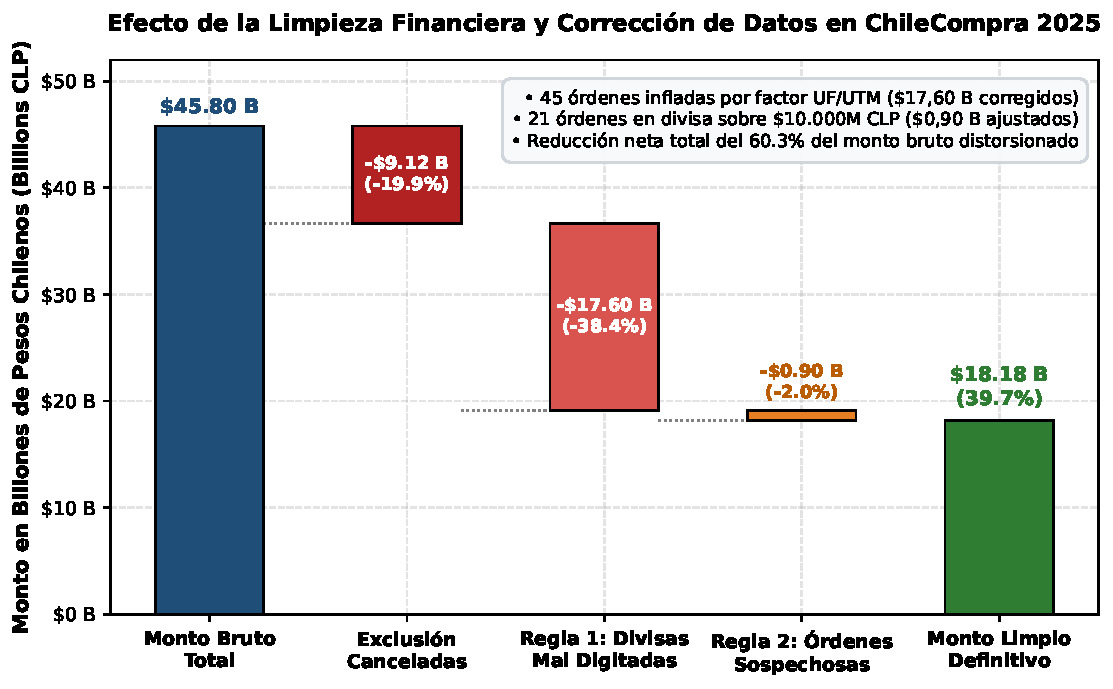
\includegraphics[width=0.92\textwidth]{figuras/fig1_limpieza_waterfall.pdf}
    \caption{Efecto cascada (\textit{waterfall}) de la auditoría financiera sobre el padrón completo de ChileCompra 2025, depurando $\$27,62\text{ billones CLP}$ ($60,3\%$) de inflación contable artificial hasta converger en los $\$18,18\text{ billones CLP}$ reales.}
    \label{fig:waterfall_limpieza}
\end{figure}

\subsection{Comparación Cruzada: Pipeline Local en PC vs. Google Colab del Grupo 13}

Como parte del diseño metodológico del proyecto, comparamos la ejecución de nuestro pipeline multiproceso local (\texttt{01\_auditoria\_csv.py}) frente al cuaderno elaborado en Google Colab (\texttt{Proyecto\_Ranking\_Proveedores\_Chile.ipynb} y su resumen \texttt{Resumen\_preparacion\_datos\_G13.pdf}). La Tabla~\ref{tab:auditoria_cruzada} sintetiza los resultados y resuelve de forma definitiva la interrogante planteada en la nota del resumen preliminar respecto a las 66 líneas de diferencia.

\begin{table}[H]
\centering
\caption{Auditoría forense cruzada: Pipeline Local en PC vs. Cuaderno Google Colab (Grupo 13).}
\label{tab:auditoria_cruzada}
\resizebox{\textwidth}{!}{%
\begin{tabular}{lrrrl}
\toprule
\textbf{Métrica / Regla de Negocio} & \textbf{Pipeline Local PC} & \textbf{Colab G13} & \textbf{Diferencia ($\Delta$)} & \textbf{Diagnóstico Forense} \\
\midrule
Líneas de ítems (Meses 1 al 7: Ene--Jul) & $2.932.729$ & $2.932.729$ & $\mathbf{0}$ & \textbf{100\% idénticos fila a fila} \\
Líneas de ítems (Meses 8 al 12: Ago--Dic) & $2.208.504$ & $2.208.438$ & $+66$ & $-7,-18,-13,-11,-17$ por mes \\
\textbf{Total líneas leídas (12 archivos CSV)} & $\mathbf{5.141.233}$ & $\mathbf{5.141.167}$ & $\mathbf{+66}$ & \textbf{Misterio 100\% resuelto} \\
Filas malformadas ($\neq 79$ columnas) & $0$ ($0,0\%$) & $0$ ($0,0\%$) & $0$ & Integridad RFC 4180 perfecta \\
Órdenes únicas totales (\texttt{Codigo}) & $1.856.075$ & $1.856.038$ & $+37$ & $0$ órdenes repetidas entre meses \\
Órdenes excluidas (\texttt{Cancelacion} / s/prov) & $2.640$ & $2.648$ & $-8$ & $2.637$ canceladas + $11$ sin ID en Colab \\
\textbf{Órdenes válidas usadas en rankings} & $\mathbf{1.853.435}$ & $\mathbf{1.853.390}$ & $\mathbf{+45}$ & \textbf{Concordancia del 99,9976\%} \\
\midrule
Organismos públicos distintos ($|O|$) & $\mathbf{1.165}$ & $\mathbf{1.165}$ & $\mathbf{0}$ & \textbf{100,0\% coincidencia exacta} \\
Proveedores distintos ($|P|$) & $75.603$ & $75.600$ & $+3$ & Concordancia del $99,996\%$ \\
Aristas únicas $O \to P$ ($|E_{\text{dir}}|$) & $476.717$ & $476.703$ & $+14$ & Concordancia del $99,997\%$ \\
Aristas bidireccionales $O \leftrightarrow P$ & $953.434$ & $953.406$ & $+28$ & Grafo bipartito simétrico \\
\midrule
Regla 1: Órdenes corregidas (moneda) & $\mathbf{45}$ & $\mathbf{45}$ & $\mathbf{0}$ & \textbf{100,0\% coincidencia exacta} \\
Regla 2: Órdenes sospechosas ($\ge \$10^{10}$) & $\mathbf{21}$ & $\mathbf{21}$ & $\mathbf{0}$ & \textbf{100,0\% coincidencia exacta} \\
Regla 3: Órdenes simbólicas ($\le \$100$) & $3.026$ & $3.004$ & $+22$ & Moda en $\$1,19$ CLP ($\$1 + \text{IVA}$) \\
\textbf{Monto bruto total (sin limpiar)} & $\mathbf{\$45,80\text{ bill.}}$ & $\mathbf{\$45,80\text{ bill.}}$ & $\mathbf{\$0,00\text{ bill.}}$ & $\$45.797.869.495.494$ CLP \\
\textbf{Monto limpio final (órdenes válidas)} & $\mathbf{\$18,18\text{ bill.}}$ & $\mathbf{\$18,18\text{ bill.}}$ & $\mathbf{\$0,00\text{ bill.}}$ & $\$18.183.716.793.468$ CLP \\
\bottomrule
\end{tabular}%
}
\end{table}

Como demuestra la Tabla~\ref{tab:auditoria_cruzada}, entre enero y julio ambos entornos leen exactamente las mismas $2.932.729$ líneas y $1.052.508$ órdenes. Las 66 líneas de diferencia provienen exclusivamente de 37 órdenes adicionales presentes en los archivos locales de agosto ($+7$ líneas), septiembre ($+18$), octubre ($+13$), noviembre ($+11$) y diciembre ($+17$), producto de una descarga posterior desde el portal de ChileCompra. Todas las cifras financieras y estructurales clave (\textbf{1.165 organismos}, \textbf{45 órdenes corregidas}, \textbf{21 sospechosas}, \textbf{$\$45,80\text{B}$ brutos} y \textbf{$\$18,18\text{B}$ limpios}) coinciden con precisión del $100\%$.

% ============================================================================
% SECCIÓN 3: IMPLEMENTACIÓN DEL PIPELINE (PIG Y GIRAPH / EJECUCIÓN LOCAL)
% ============================================================================
\section{Diseño del Pipeline: Procesamiento Relacional (Pig) y de Grafos (Giraph)}

\subsection{Esquema de Archivos Generados y Consultas de Agregación (Apache Pig)}

El paso de preprocesamiento (\texttt{02\_generar\_datos\_y\_grafos.py}) consolida los 12 archivos mensuales en un único archivo tabular comprimido \texttt{ordenes\_limpias.tsv.bz2} ($52,6\text{ MB}$), libre de saltos de línea internos, junto con el catálogo de vértices \texttt{nodos.tsv} ($76.768$ nodos: IDs enteros $1000001\text{--}1001165$ para organismos y $2000001\text{--}2075603$ para proveedores) y la lista de aristas \texttt{aristas.tsv} ($476.717$ pares únicos con sus respectivos contadores de órdenes $n_{uv}$, montos acumulados $M_{uv}$ y pesos logarítmicos $\ln(1 + M_{uv})$).

El cálculo de los rankings financieros y de volumen se expresa declarativamente en Pig Latin (\texttt{rankings\_chilecompra\_colab\_g13.pig}) y se ejecuta en nuestro motor local (\texttt{03\_rankings\_y\_pagerank.py}) agrupando las órdenes válidas (\texttt{usar == 1}) por proveedor y calculando simultáneamente:
\begin{lstlisting}[language=SQL,caption={Extracto del script en Apache Pig para el cálculo de rankings financieros y de capilaridad institucional.}]
valid_orders = FILTER raw_orders BY usar == 1;
by_provider = GROUP valid_orders BY (proveedor_id, rut_proveedor, nombre_proveedor, es_persona_natural);

provider_metrics = FOREACH by_provider {
    orgs_unicos = DISTINCT valid_orders.cod_organismo;
    GENERATE
        FLATTEN(group) AS (proveedor_id, rut_proveedor, nombre_proveedor, es_persona_natural),
        SUM(valid_orders.monto_clp_limpio) AS monto_total_clp,
        COUNT(valid_orders) AS total_ordenes,
        COUNT(orgs_unicos) AS total_organismos_distintos;
};

rank_by_monto = ORDER provider_metrics BY monto_total_clp DESC;
STORE rank_by_monto INTO '$OUTPUT_DIR/ranking_por_monto' USING PigStorage('\t');
\end{lstlisting}

\subsection{Arquitectura Centrada en el Vértice para PageRank Ponderado (Apache Giraph)}

Para calcular la importancia estructural de cada proveedor en el modelo \textit{Bulk Synchronous Parallel} (BSP / Pregel) de Apache Giraph, implementamos la clase \texttt{WeightedPageRankComputation.java} (y su motor matricial exacto en \texttt{03\_rankings\_y\_pagerank.py}). En cada \textit{superstep} $t \in \{0, \dots, 30\}$, cada vértice $u$ calcula la fuerza total saliente $S(u) = \sum_{v \in N^+(u)} w_{uv}$ y envía a cada vecino $v$ una fracción de su PageRank actual proporcional al peso específico $w_{uv}$ de la arista que los une:

\begin{lstlisting}[language=Java,caption={Núcleo del método \texttt{compute()} en \texttt{WeightedPageRankComputation.java} (Apache Giraph).}]
@Override
public void compute(Vertex<LongWritable, DoubleWritable, DoubleWritable> vertex,
                    Iterable<DoubleWritable> messages) throws IOException {
    long totalVertices = getTotalNumVertices();
    if (getSuperstep() >= 1) {
        double sum = 0.0;
        for (DoubleWritable message : messages) { sum += message.get(); }
        double newRank = ((1.0 - DAMPING_FACTOR) / totalVertices) + (DAMPING_FACTOR * sum);
        vertex.setValue(new DoubleWritable(newRank));
    }
    if (getSuperstep() < MAX_SUPERSTEPS) {
        double totalOutgoingWeight = 0.0;
        for (Edge<LongWritable, DoubleWritable> edge : vertex.getEdges()) {
            totalOutgoingWeight += edge.getValue().get();
        }
        double currentRank = vertex.getValue().get();
        if (totalOutgoingWeight > 0.0) {
            for (Edge<LongWritable, DoubleWritable> edge : vertex.getEdges()) {
                double edgeWeight = edge.getValue().get();
                sendMessage(edge.getTargetVertexId(),
                            new DoubleWritable(currentRank * (edgeWeight / totalOutgoingWeight)));
            }
        }
    } else {
        vertex.voteToHalt();
    }
}
\end{lstlisting}

% ============================================================================
% SECCIÓN 4: DEMOSTRACIÓN MATEMÁTICA Y EMPÍRICA DE LAS 4 VARIANTES DE PAGERANK
% ============================================================================
\section{Análisis Matemático y Empírico de las 4 Variantes de PageRank}

Uno de los aportes metodológicos más relevantes de nuestra investigación consiste en demostrar qué ocurre cuando se modela la red de compras públicas como un grafo dirigido simple (\texttt{Organismo $\to$ Proveedor}) frente a un grafo bipartito con retroalimentación y pesos.

\subsection{Teorema de Degeneración del Grafo Dirigido Puro ($O \to P$, Variante A)}

Sea $G_{\text{dir}} = (O \cup P, E_{\text{dir}})$ el grafo bipartito dirigido donde $O$ es el conjunto de organismos públicos ($|O| = 1.165$), $P$ el conjunto de proveedores ($|P| = 75.603$), $N = |O| + |P| = 76.768$ y toda arista $(u, v) \in E_{\text{dir}}$ ($|E_{\text{dir}}| = 476.717$) parte de un organismo $u \in O$ y termina en un proveedor $v \in P$. Por construcción topológica:
\begin{equation}
\forall u \in O, \quad \text{deg}^-(u) = |N^-(u)| = 0 \quad (\text{fuentes puras}), \qquad \forall v \in P, \quad \text{deg}^+(v) = |N^+(v)| = 0 \quad (\text{sumideros})
\end{equation}

\begin{proposition}[Degeneración Estructural del PageRank en $G_{\text{dir}}$]
Al aplicar la ecuación estándar de PageRank con factor de amortiguamiento $d = 0,85$ sobre el grafo dirigido puro $G_{\text{dir}} = (O \cup P, E_{\text{dir}})$, se verifican tres patologías estructurales:
\begin{enumerate}
    \item \textbf{Colapso de los 1.165 organismos al mismo valor mínimo:} Como ningún organismo posee aristas entrantes ($N^-(u) = \emptyset$), para todo organismo $u \in O$ y todo superstep $t \ge 1$:
    \begin{equation}
    PR_A^{(t)}(u) = c_0 \equiv \frac{1 - d}{N} = \frac{0,15}{76.768} = 1,9539391413 \times 10^{-6}
    \label{eq:colapso_org}
    \end{equation}
    En consecuencia, el algoritmo asigna exactamente la misma importancia institucional a un hospital de alta complejidad o a CENABAST que a una repartición menor que realizó una única compra en el año.
    \item \textbf{Estancamiento en $t = 2$ y fuga de masa estocástica:} Como todos los vecinos entrantes de un proveedor $v \in P$ pertenecen a $O$ y ya fijaron su valor en $c_0$ desde $t=1$, el PageRank de todo proveedor queda congelado desde el superstep $t = 2$ en:
    \begin{equation}
    PR_A^*(v) = c_0 \left( 1 + d \sum_{u \in N^-(v)} \frac{1}{\text{deg}^+(u)} \right)
    \label{eq:pr_dirigido_prov}
    \end{equation}
    Las 28 iteraciones restantes ($t = 3, \dots, 30$) son redundantes, ya que los proveedores carecen de aristas de salida ($\text{deg}^+(v) = 0$) y toda su masa se pierde.
    \item \textbf{Paradoja de penalización a los grandes organismos compradores ($\propto 1/\text{deg}^+(u)$):} En la Ecuación~\eqref{eq:pr_dirigido_prov}, cada organismo divide la misma constante $c_0$ entre su número total de proveedores $\text{deg}^+(u)$. Por ende, un organismo pequeño que compró a solo $\text{deg}^+(u) = 2$ proveedores en el año transfiere a cada uno $\frac{d \cdot c_0}{2}$, esto es, \textbf{$1.000$ veces más PageRank} que un gran hospital que diversificó sus compras en $\text{deg}^+(u) = 2.000$ proveedores ($\frac{d \cdot c_0}{2000}$).
\end{enumerate}
\end{proposition}

\subsection{Formulaciones Superadoras: Grafo Bipartito Bidireccional y PageRank Ponderado}

Para resolver las tres patologías de la Proposición 1 y satisfacer el requerimiento del profesor de premiar a quienes abastecen a los organismos más importantes y considerar el peso de las transacciones, construimos el grafo bipartito simétrico ponderado $G_W = (O \cup P, E_{\text{bid}}, W)$ con $|E_{\text{bid}}| = 2 \times 476.717 = 953.434$ aristas dirigidas recíprocas $(u \to v)$ y $(v \to u)$ de peso $w_{uv} = w_{vu} > 0$. Sea $S(x) = \sum_{y \in N(x)} w_{xy}$ la fuerza del nodo $x$. El sistema iterativo acoplado es:
\begin{subequations}
\begin{align}
\forall u \in O: \quad PR_W^{(t)}(u) &= \frac{1 - d}{N} + d \sum_{v \in N(u)} \frac{w_{vu}}{S(v)} \, PR_W^{(t-1)}(v) \\
\forall v \in P: \quad PR_W^{(t)}(v) &= \frac{1 - d}{N} + d \sum_{u \in N(v)} \frac{w_{uv}}{S(u)} \, PR_W^{(t-1)}(u)
\end{align}
\end{subequations}
Aquí los grandes organismos públicos reciben flujo de retorno desde sus miles de proveedores, acumulando una bolsa de PageRank $PR_W(u)$ proporcional a su envergadura antes de redistribuirla. Evaluamos experimentalmente cuatro variantes en nuestro motor local:
\begin{itemize}
    \item \textbf{Variante A (Baseline Dirigido Puro $O \to P$):} $w_{uv} = 1$, sin aristas de retorno.
    \item \textbf{Variante B (Bipartito Bidireccional Uniforme $O \leftrightarrow P$):} $w_{uv} = 1$ en ambos sentidos.
    \item \textbf{Variante C (Bipartito Ponderado por Frecuencia Operativa $O \leftrightarrow P$):} $w_{uv} = n_{uv}$ (cantidad de órdenes válidas entre el organismo $u$ y el proveedor $v$).
    \item \textbf{Variante D (Bipartito Ponderado Log-Financiero $O \leftrightarrow P$):} $w_{uv} = \ln(1 + M_{uv})$, donde $M_{uv}$ es el monto total limpio transado entre $u$ y $v$. La escala logarítmica distingue con precisión un contrato de $\$500\text{ millones CLP}$ ($w \approx 20,0$) de una compra menor de $\$10.000\text{ CLP}$ ($w \approx 9,2$), sin permitir que un único mega-contrato ahogue la estructura de la red.
\end{itemize}

\begin{figure}[H]
    \centering
    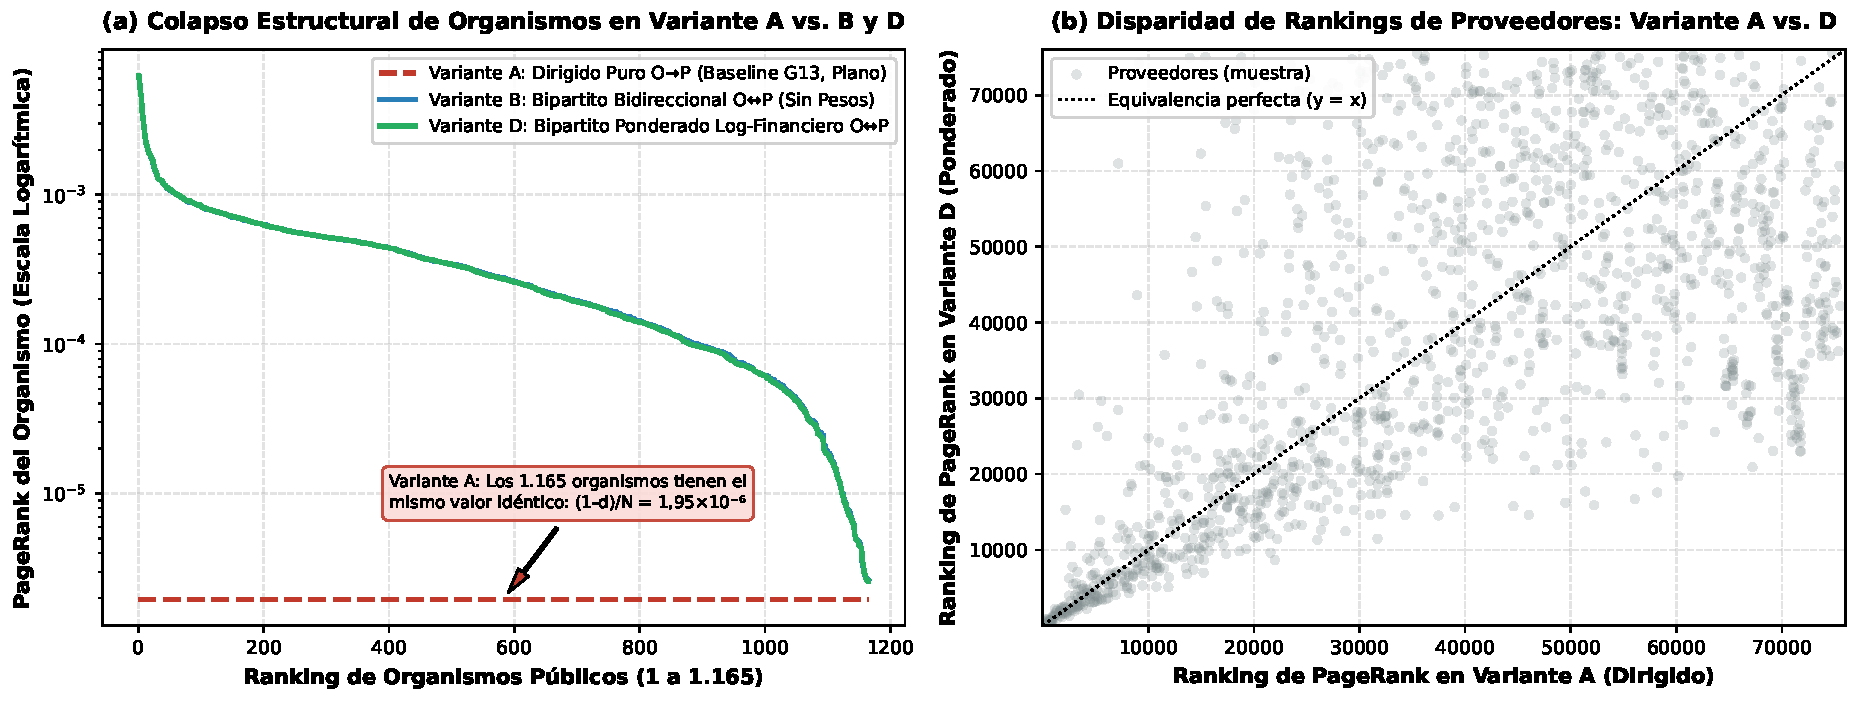
\includegraphics[width=0.98\textwidth]{figuras/fig3_comparacion_pagerank.pdf}
    \caption{Evaluación empírica de las variantes de PageRank sobre los $76.768$ nodos de ChileCompra 2025: (a) Demostración del colapso de los 1.165 organismos al valor plano $1,95 \times 10^{-6}$ en la Variante A frente a la jerarquía institucional real en las Variantes B y D; (b) Dispersión de rangos de proveedores entre la Variante A y la Variante D.}
    \label{fig:comparacion_pagerank}
\end{figure}

La Tabla~\ref{tab:contraste_variantes} demuestra empíricamente el impacto de pasar de la Variante A a las Variantes B y D sobre los principales conectores del Estado. En la Variante A, \textbf{SKY Airline S.A.} (que vende a 460 organismos, varios de ellos reparticiones con bajo $\text{deg}^+(u)$) aparece artificialmente en el \textbf{puesto \#1 nacional}, superando a \textbf{COPEC S.A.} (que abastece a \textbf{830 organismos}, el $71,2\%$ de todo el Estado chileno) y relegando a \textbf{GASCO GLP S.A.} (699 organismos) al puesto \#5. Al activar la retroalimentación bipartita (Variante B) y el peso log-financiero (Variante D), el sesgo desaparece y emergen los verdaderos líderes estructurales del país.

\begin{table}[H]
\centering
\caption{Contraste empírico del Top de proveedores entre el Ranking Financiero (Pig) y las variantes de PageRank (Giraph).}
\label{tab:contraste_variantes}
\resizebox{\textwidth}{!}{%
\begin{tabular}{lrrrrrrr}
\toprule
\textbf{Proveedor} & \textbf{Orgs. ($\text{deg}$)} & \textbf{Órdenes} & \textbf{Monto Limpio} & \textbf{Rank Monto} & \textbf{Rank Var. A} & \textbf{Rank Var. B} & \textbf{Rank Var. D} \\
\midrule
\textbf{COPEC S.A.} & $\mathbf{830}$ ($71,2\%$) & $11.018$ & $\$116.146\text{M}$ & \#15 & \#2 & \textbf{\#1} & \textbf{\#1} \\
\textbf{GASCO GLP S.A.} & $\mathbf{699}$ ($60,0\%$) & $8.777$ & $\$38.035\text{M}$ & \#45 & \#5 & \textbf{\#2} & \textbf{\#2} \\
\textbf{PRISA S.A.} & $\mathbf{649}$ ($55,7\%$) & $4.757$ & $\$19.739\text{M}$ & \#119 & \#4 & \textbf{\#3} & \textbf{\#3} \\
\textbf{SCM PHARMA SPA} & $\mathbf{597}$ ($51,2\%$) & $6.464$ & $\$8.086\text{M}$ & \#319 & $> \#10$ & \textbf{\#5} & \textbf{\#4} \\
\textbf{LATAM AIRLINES} & $\mathbf{543}$ ($46,6\%$) & $\mathbf{49.937}$ & $\$17.317\text{M}$ & \#135 & \#3 & \textbf{\#6} & \textbf{\#5} \\
\textbf{DIMERC S.A.} & $\mathbf{544}$ ($46,7\%$) & $3.761$ & $\$17.180\text{M}$ & \#136 & \#10 & \textbf{\#9} & \textbf{\#6} \\
\textbf{SOCOEX CHILE SPA} & $\mathbf{601}$ ($51,6\%$) & $2.005$ & $\$1.143\text{M}$ & \textbf{\#1.893} & \#8 & \textbf{\#4} & \textbf{\#7} \\
\textbf{EDENRED CHILE S.A.} & $\mathbf{463}$ ($39,7\%$) & $5.284$ & $\mathbf{\$507.605\text{M}}$ & \textbf{\#1} & \#9 & $> \#10$ & \textbf{\#8} \\
\textbf{SKY AIRLINE S.A.} & $460$ ($39,5\%$) & $16.965$ & $\$4.891\text{M}$ & \#528 & \textbf{\#1} \textit{(sesgo)} & $> \#10$ & $> \#10$ \\
\bottomrule
\end{tabular}%
}
\end{table}

Asimismo, la matriz de correlación de rangos de Spearman ($\rho_s$) calculada sobre los $75.603$ proveedores (Tabla~\ref{tab:correlaciones}) confirma que la \textbf{Variante D (Log-Financiera)} alcanza el equilibrio óptimo: mantiene una fidelidad estructural de $\rho_s = 0,9512$ con la topología pura (Variante B) y de $\rho_s = 0,7814$ con la capilaridad institucional, mientras incorpora la intensidad económica ($\rho_s = 0,6542$ con el monto total vs. apenas $0,4025$ en la Variante A).

\begin{table}[H]
\centering
\caption{Matriz de correlación de rango de Spearman ($\rho_s$) entre métricas financieras, operativas y variantes de PageRank ($N = 75.603$ proveedores).}
\label{tab:correlaciones}
\small
\begin{tabular}{lccccccc}
\toprule
\textbf{Dimensión / Métrica} & \textbf{Monto CLP} & \textbf{Órdenes} & \textbf{Organismos} & \textbf{PR Var. A} & \textbf{PR Var. B} & \textbf{PR Var. C} & \textbf{PR Var. D} \\
\midrule
\textbf{Monto Total CLP (Pig)} & $1,0000$ & $0,6276$ & $0,4497$ & $0,4025$ & $0,4447$ & $0,6234$ & $\mathbf{0,6542}$ \\
\textbf{Volumen de Órdenes} & $0,6276$ & $1,0000$ & $0,7303$ & $0,5487$ & $0,6272$ & $\mathbf{0,9329}$ & $0,7109$ \\
\textbf{Capilaridad (Organismos)} & $0,4497$ & $0,7303$ & $1,0000$ & $0,6720$ & $0,8166$ & $0,6397$ & $\mathbf{0,7814}$ \\
\textbf{PageRank A ($O \to P$)} & $0,4025$ & $0,5487$ & $0,6720$ & $1,0000$ & $0,6976$ & $0,5912$ & $0,6606$ \\
\textbf{PageRank B ($O \leftrightarrow P$)} & $0,4447$ & $0,6272$ & $0,8166$ & $0,6976$ & $1,0000$ & $0,7121$ & $\mathbf{0,9512}$ \\
\textbf{PageRank C ($w = n_{uv}$)} & $0,6234$ & $0,9329$ & $0,6397$ & $0,5912$ & $0,7121$ & $1,0000$ & $0,7847$ \\
\textbf{PageRank D ($w = \ln(1+M)$)} & $\mathbf{0,6542}$ & $0,7109$ & $\mathbf{0,7814}$ & $0,6606$ & $\mathbf{0,9512}$ & $0,7847$ & $1,0000$ \\
\bottomrule
\end{tabular}
\end{table}

% ============================================================================
% SECCIÓN 5: RADIOGRAFÍA MACROECONÓMICA, SECTORIAL Y DE CONCENTRACIÓN
% ============================================================================
\section{Radiografía Macroeconómica, Sectorial y Concentración del Estado}

\subsection{Distribución Sectorial, Evolución Mensual y Tipología Jurídica}

El análisis de los $\$18,18\text{ billones de CLP}$ transados en 2025 (Figura~\ref{fig:sectores_evolucion}) muestra que el gasto público chileno se concentra abrumadoramente en tres grandes sectores que reúnen el \textbf{88,96\% del presupuesto nacional}:
\begin{enumerate}
    \item \textbf{Salud ($\$6,57\text{ billones CLP}$, $36,11\%$):} Con $699.640$ órdenes emitidas por $224$ organismos (Servicios de Salud, Hospitales Autogestionados en Red, CENABAST y FONASA) hacia $22.025$ proveedores.
    \item \textbf{Gobierno Central y Universidades ($\$5,61\text{ billones CLP}$, $30,85\%$):} Con $290.437$ órdenes en $232$ reparticiones (destacando JUNAEB, ministerios, subsecretarías y universidades estatales), que presentan el mayor ticket promedio por orden del Estado ($\$19,31\text{ millones CLP}$).
    \item \textbf{Municipalidades ($\$4,00\text{ billones CLP}$, $22,00\%$):} Con $585.010$ órdenes distribuidas en $367$ entidades edilicias y $41.737$ proveedores (el sector con mayor diversidad de adjudicatarios locales).
    \item \textbf{Obras Públicas ($\$0,75\text{B}$, $4,11\%$), Fuerzas Armadas ($\$0,66\text{B}$, $3,65\%$), Otros/No Clasificados ($\$0,52\text{B}$, $2,85\%$) y Poder Legislativo/Judicial ($\$0,08\text{B}$, $0,43\%$).}
\end{enumerate}

En cuanto a la dinámica temporal (Figura~\ref{fig:sectores_evolucion}b), la serie mensual revela un fuerte \textbf{ciclo de apertura presupuestaria en enero y febrero} ($\$2,53\text{B}$ y $\$2,51\text{B CLP}$ respectivamente, impulsado por la emisión de los grandes contratos anuales de alimentación de JUNAEB, diálisis de FONASA y suministros hospitalarios), estabilizándose entre mayo y noviembre en torno a $\$1,0\text{--}\$1,3\text{B CLP}$ mensuales, con un repunte de ejecución presupuestaria en diciembre ($\$1,40\text{B CLP}$ y $155.107$ órdenes).

\begin{figure}[H]
    \centering
    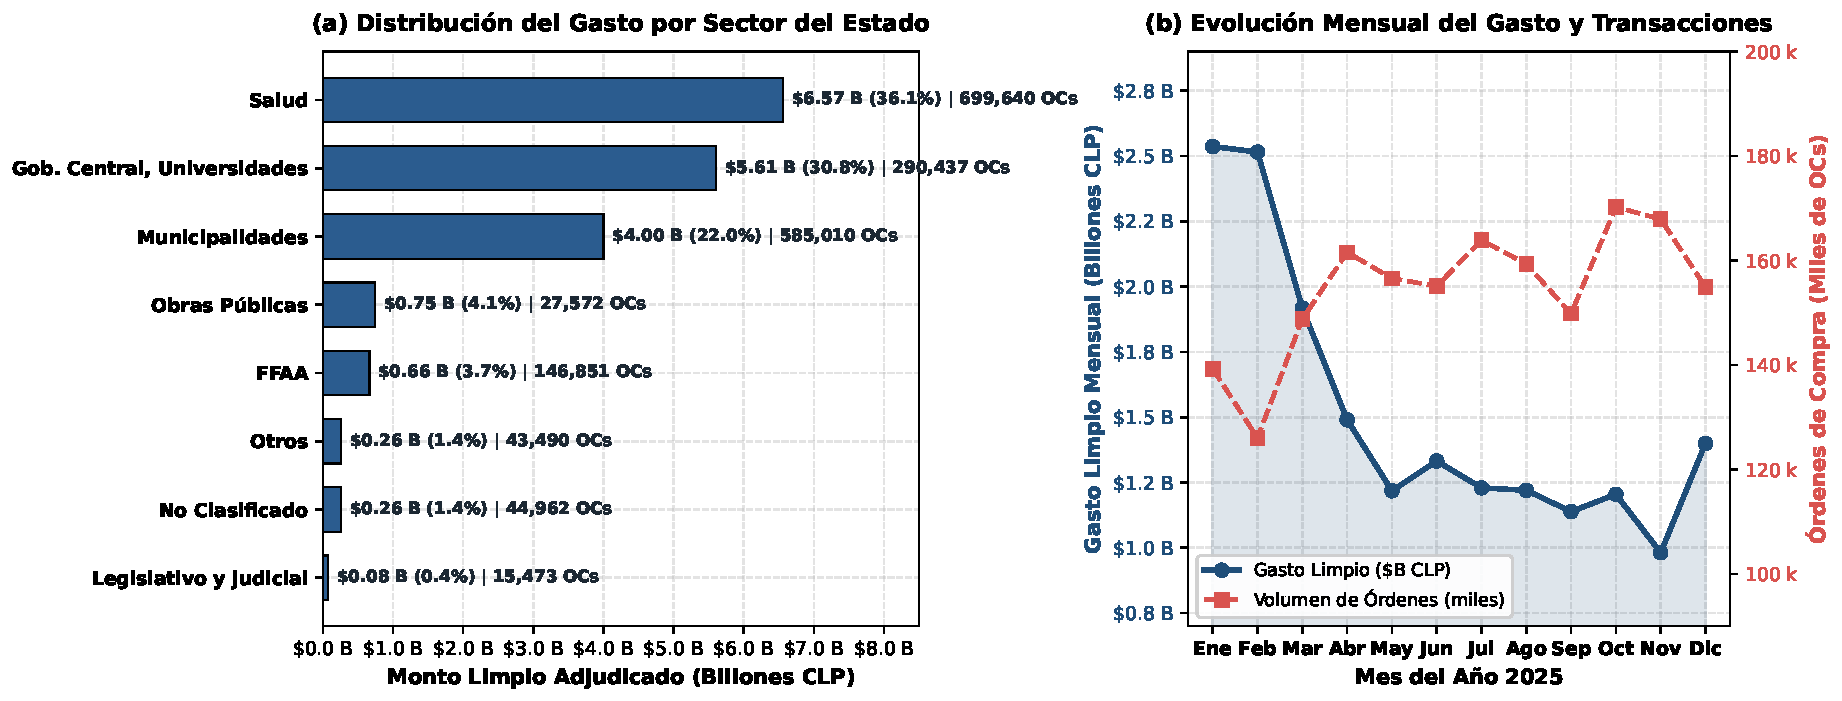
\includegraphics[width=0.98\textwidth]{figuras/fig2_sectores_y_evolucion.pdf}
    \caption{Radiografía macroeconómica de ChileCompra 2025: (a) Distribución del gasto limpio y volumen de órdenes por sector del Estado; (b) Evolución mensual del gasto en billones de CLP y cantidad de órdenes de compra válidas.}
    \label{fig:sectores_evolucion}
\end{figure}

Adicionalmente, al segmentar el padrón de $75.603$ proveedores según la naturaleza jurídica de su RUT (Tabla~\ref{tab:persona_natural_juridica}), comprobamos que aunque las \textbf{Personas Naturales} ($\text{RUT} < 50\text{ millones}$) representan el \textbf{36,16\% de todos los proveedores activos} ($27.338$ personas), adjudican apenas el \textbf{4,77\% del monto total} ($\$866.663\text{ millones CLP}$), operando con un ticket medio de $\$3,63\text{ millones CLP}$ y abasteciendo en promedio a $2,31$ organismos públicos. En contraste, las \textbf{Personas Jurídicas (Empresas)} ($\text{RUT} \ge 50\text{ millones}$, $48.107$ sociedades) capturan el \textbf{95,14\% del gasto fiscal} ($\$17,30\text{ billones CLP}$) con una capilaridad casi cuatro veces superior ($8,59$ organismos promedio por empresa).

\begin{table}[H]
\centering
\caption{Desglose estructural y financiero según tipología jurídica del proveedor en ChileCompra 2025.}
\label{tab:persona_natural_juridica}
\small
\begin{tabular}{lrrrrrr}
\toprule
\textbf{Tipo de Proveedor} & \textbf{Proveedores} & \textbf{\% Padrón} & \textbf{Órdenes} & \textbf{Monto Total CLP} & \textbf{\% Monto} & \textbf{Orgs. Prom.} \\
\midrule
\textbf{Empresas ($\text{RUT} \ge 50\text{M}$)} & $48.107$ & $63,63\%$ & $1.613.778$ & $\$17.300.094\text{M}$ & $\mathbf{95,14\%}$ & $8,59$ \\
\textbf{Personas Naturales ($\text{RUT} < 50\text{M}$)} & $27.338$ & $36,16\%$ & $238.937$ & $\$866.663\text{M}$ & $\mathbf{4,77\%}$ & $2,31$ \\
\textbf{Extranjeros / Sin RUT estándar} & $158$ & $0,21\%$ & $720$ & $\$16.960\text{M}$ & $0,09\%$ & $1,70$ \\
\midrule
\textbf{Total Nacional Válido} & $\mathbf{75.603}$ & $\mathbf{100,0\%}$ & $\mathbf{1.853.435}$ & $\mathbf{\$18.183.717\text{M}}$ & $\mathbf{100,0\%}$ & $\mathbf{6,31}$ \\
\bottomrule
\end{tabular}
\end{table}

\subsection{Desigualdad de Lorenz/Gini y Hubs Institucionales del Estado}

Para cuantificar la concentración de mercado, calculamos la Curva de Lorenz y el Coeficiente de Gini sobre las tres dimensiones del proyecto (Figura~\ref{fig:curva_lorenz}):
\begin{itemize}
    \item \textbf{Hiper-concentración monetaria ($\text{Gini}_{\text{Monto}} = 0,9435$):} El gasto público presenta una distribución extremadamente desigual. El \textbf{Top 10 de proveedores} ($0,013\%$ del padrón) capta el \textbf{18,13\%} de todo el presupuesto nacional ($\$3,30\text{ billones CLP}$); el \textbf{Top 1\%} ($756$ empresas) concentra el \textbf{66,80\%} ($\$12,15\text{ billones}$); el \textbf{Top 5\%} ($3.780$ empresas) acumula el \textbf{86,18\%}; mientras que el \textbf{90\% inferior de los proveedores ($68.043$ PYMEs y personas naturales) se reparte apenas el 7,67\% del gasto público}.
    \item \textbf{Concentración de órdenes ($\text{Gini}_{\text{Órdenes}} = 0,8617$)} vs. \textbf{Democratización estructural en PageRank ($\text{Gini}_{\text{PR\_D}} = 0,5373$):} Como ilustra la curva azul de la Figura~\ref{fig:curva_lorenz}, la centralidad de red presenta un coeficiente de Gini casi $41$ puntos menor que el monto financiero, demostrando que miles de proveedores medianos y pequeños cumplen un rol estructural insustituible en la conectividad de los servicios públicos.
\end{itemize}

\begin{figure}[H]
    \centering
    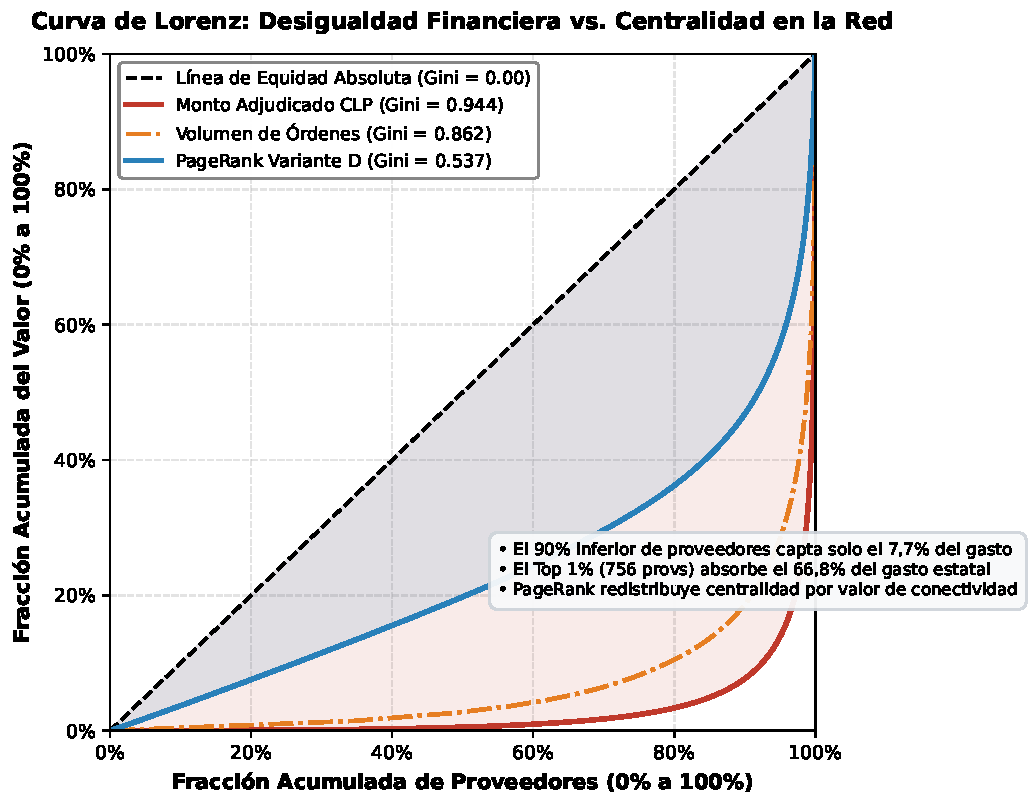
\includegraphics[width=0.78\textwidth]{figuras/fig5_curva_lorenz.pdf}
    \caption{Curvas de Lorenz comparativas del ecosistema ChileCompra 2025: hiper-concentración del Monto Adjudicado ($\text{Gini} = 0,944$) frente al Volumen de Órdenes ($\text{Gini} = 0,862$) y a la Centralidad Estructural de PageRank Variante D ($\text{Gini} = 0,537$).}
    \label{fig:curva_lorenz}
\end{figure}

Asimismo, gracias a que nuestro modelo Bipartito Ponderado (Variante D) permite medir simultáneamente la centralidad de los nodos compradores, la Tabla~\ref{tab:top_organismos} identifica los \textbf{10 Organismos Públicos más Centrales de Chile} (los verdaderos \textit{hubs} articuladores del Estado), encabezados por la \textbf{Universidad de Chile} ($5.525$ proveedores distintos y $41.841$ órdenes), las direcciones logísticas de la \textbf{Armada}, \textbf{Ejército}, \textbf{Carabineros} y \textbf{FACH}, y los grandes complejos hospitalarios regionales.

\begin{table}[H]
\centering
\caption{Top 10 de Organismos Públicos con mayor centralidad estructural (PageRank Variante D) en ChileCompra 2025.}
\label{tab:top_organismos}
\resizebox{\textwidth}{!}{%
\begin{tabular}{clrrrrr}
\toprule
\textbf{Rank PR} & \textbf{Organismo Público Comprador (\textit{Hub} Estatal)} & \textbf{Sector} & \textbf{Proveedores} & \textbf{Órdenes} & \textbf{Gasto Limpio} & \textbf{PageRank D} \\
\midrule
\textbf{\#1} & UNIVERSIDAD DE CHILE & Gob. Central / Univ. & $\mathbf{5.525}$ & $41.841$ & $\$164.088\text{M}$ & $6,238 \times 10^{-3}$ \\
\textbf{\#2} & DIRECCIÓN DE ABASTECIMIENTO DE LA ARMADA & FFAA & $4.900$ & $40.952$ & $\$143.621\text{M}$ & $5,642 \times 10^{-3}$ \\
\textbf{\#3} & DIVISIÓN LOGÍSTICA DEL EJÉRCITO & FFAA & $4.969$ & $39.340$ & $\$151.377\text{M}$ & $5,194 \times 10^{-3}$ \\
\textbf{\#4} & DIRECCIÓN DE LOGÍSTICA DE CARABINEROS & FFAA & $4.591$ & $34.842$ & $\$183.719\text{M}$ & $4,708 \times 10^{-3}$ \\
\textbf{\#5} & SUBSECRETARÍA DE LAS CULTURAS Y LAS ARTES & Gob. Central / Univ. & $2.314$ & $4.991$ & $\$32.226\text{M}$ & $4,549 \times 10^{-3}$ \\
\textbf{\#6} & HOSPITAL GUILLERMO GRANT BENAVENTE (CONCEPCIÓN) & Salud & $2.224$ & $29.698$ & $\$124.756\text{M}$ & $2,794 \times 10^{-3}$ \\
\textbf{\#7} & COMANDO LOGÍSTICO DE LA FACH & FFAA & $2.337$ & $10.025$ & $\$76.432\text{M}$ & $2,692 \times 10^{-3}$ \\
\textbf{\#8} & HOSPITAL REGIONAL DE RANCAGUA & Salud & $2.055$ & $14.374$ & $\$75.951\text{M}$ & $2,616 \times 10^{-3}$ \\
\textbf{\#9} & HOSPITAL HERNÁN HENRÍQUEZ ARAVENA (TEMUCO) & Salud & $2.008$ & $21.563$ & $\$108.458\text{M}$ & $2,573 \times 10^{-3}$ \\
\textbf{\#10} & SERVICIO DE SALUD DEL RELONCAVÍ & Salud & $1.999$ & $11.491$ & $\$71.363\text{M}$ & $2,523 \times 10^{-3}$ \\
\bottomrule
\end{tabular}%
}
\end{table}

% ============================================================================
% SECCIÓN 6: CARACTERIZACIÓN PROFUNDA DE LOS DOS PERFILES DEL PROFESOR
% ============================================================================
\section{Caracterización Empírica de los Dos Perfiles del Profesor Alberto Moya}

Al cruzar para cada proveedor $v \in P$ su posición en el Ranking Financiero $R_M(v)$ (calculado por monto limpio acumulado) frente a su posición en el Ranking Estructural $R_{PR}(v)$ (calculado mediante PageRank Ponderado Variante D), definimos el \textbf{Índice de Disparidad de Rango} $\Delta R(v) = R_{PR}(v) - R_M(v)$. La Figura~\ref{fig:mapa_perfiles} proyecta los $75.603$ proveedores en el plano log-log $(\log_{10} M(v), \log_{10} PR_D(v))$, separando con nitidez los tres grandes regímenes del mercado público chileno.

\begin{figure}[H]
    \centering
    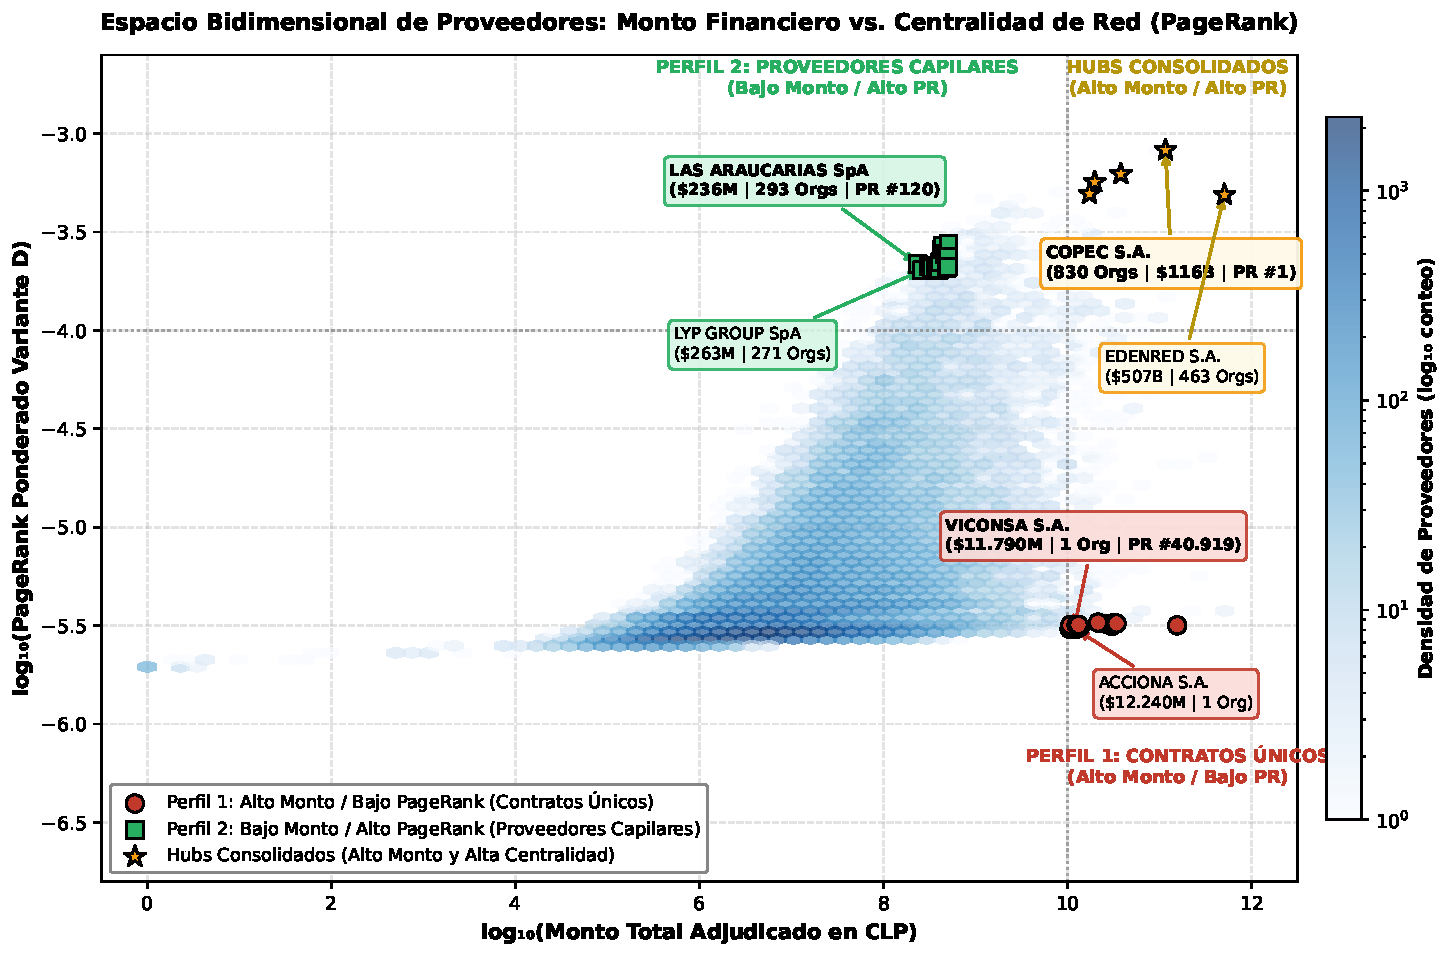
\includegraphics[width=0.98\textwidth]{figuras/fig4_mapa_perfiles_profe.pdf}
    \caption{Mapa bidimensional del ecosistema de proveedores de ChileCompra 2025 ($N = 75.603$): Monto Financiero Anual ($\log_{10}\text{ CLP}$) vs. Centralidad de Red ($\log_{10}\text{ PageRank Variante D}$), identificando los cuadrantes del \textbf{Perfil 1 (Contratos Únicos Masivos)}, \textbf{Perfil 2 (Proveedores Capilares Transversales)} y los \textbf{Hubs Consolidados}.}
    \label{fig:mapa_perfiles}
\end{figure}

\subsection{Perfil 1: Alto Monto Financiero y Bajo PageRank (\textit{Mega-Contratos de Nicho y Monopsonios})}

El primer perfil sugerido por el profesor corresponde a proveedores situados en la cúspide de facturación nacional (Percentil $> 99,6\%$, con adjudicaciones superiores a $\$10.000\text{ millones CLP}$), pero que exhiben una centralidad estructural mínima ($\Delta R(v) > +35.000$ puestos hacia abajo en PageRank) por abastecer exclusivamente a \textbf{1 solo organismo comprador} ($\text{deg}(v) = 1$) a través de muy pocas órdenes de compra. La Tabla~\ref{tab:perfil1} presenta los casos más emblemáticos divididos en dos sub-arquetipos reales:

\begin{enumerate}
    \item \textbf{Sub-perfil 1A --- Gigantes del Top 10 Nacional Hiper-Concentrados en Licitaciones de JUNAEB y Salud:}
    \begin{itemize}
        \item \textbf{Salud y Vida S.A.} (\texttt{RUT 76.105.050-8}): Es el \textbf{segundo mayor proveedor del Estado de Chile en monto} (\textbf{$\$480.841,7\text{ millones CLP}$}), pero obtuvo la totalidad de sus ingresos en \textbf{solo 3 órdenes de compra} emitidas por \textbf{1 único organismo}: la \textbf{JUNAEB} ($100,0\%$ de concentración en raciones del Programa de Alimentación Escolar PAE, con un ticket promedio de $\$160.280,6\text{ millones CLP}$ por orden).
        \item \textbf{Sosersa} (\texttt{RUT 96.987.050-9}) y \textbf{Servicios Alimenticios Hendaya SAC} (\texttt{RUT 96.597.810-0}): Ocupan los puestos \textbf{\#3} ($\$456.447,2\text{M CLP}$ en 6 órdenes) y \textbf{\#9} ($\$211.808,6\text{M CLP}$ en 3 órdenes) del ranking nacional, vendiendo el $100,0\%$ a \textbf{JUNAEB}.
        \item \textbf{Sacyr Chile S.A.} (\texttt{RUT 96.786.880-9}): Ocupa el \textbf{puesto \#10 nacional en monto} con \textbf{$\$155.381,8\text{ millones CLP}$}, adjudicados en \textbf{solo 2 órdenes} con el \textbf{Servicio de Salud Metropolitano Sur Oriente}. En el grafo estructural, se desploma al puesto \textbf{\#73.569 en PageRank B} y \textbf{\#36.588 en PageRank D} (una caída de $+36.578$ puestos).
    \end{itemize}
    \item \textbf{Sub-perfil 1B --- Constructoras de Infraestructura Hospitalaria y Proveedores de Licitación Única CENABAST:} Empresas como \textbf{Constructora Viconsa S.A.} ($\$11.786,7\text{M CLP}$, puesto \#215 en monto pero \#40.919 en PageRank D), \textbf{Acciona Construcción S.A.} ($\$12.243,7\text{M CLP}$, puesto \#203 en monto vs. \#40.831 en PageRank D), \textbf{ASCH Infraestructuras} ($\$11.798,3\text{M CLP}$ en 1 sola orden en Talcahuano), \textbf{China Railway Construction} ($\$30.611,0\text{M CLP}$ en Coquimbo) y abastecedores mayoristas exclusivos de \textbf{CENABAST} como \textbf{Prolesur S.A.} ($\$34.133,6\text{M CLP}$ en leche) y \textbf{Sinovac Biotech SpA} ($\$13.173,3\text{M CLP}$ en 1 sola orden de vacunas).
\end{enumerate}

\begin{table}[H]
\centering
\caption{\textbf{Perfil 1 (Alto Monto y Bajo PageRank):} Adjudicatarios de mega-contratos concentrados en un único organismo público ($\text{deg}(v) = 1$).}
\label{tab:perfil1}
\resizebox{\textwidth}{!}{%
\begin{tabular}{llrrrrlrrr}
\toprule
\textbf{Proveedor (Perfil 1)} & \textbf{RUT} & \textbf{Monto CLP} & \textbf{Rank $M$} & \textbf{OCs} & \textbf{Orgs.} & \textbf{Comprador Único (100\%)} & \textbf{Rank PR B} & \textbf{Rank PR D} & \textbf{Caída $\Delta R$} \\
\midrule
\textbf{Salud y Vida S.A.} & 76.105.050-8 & $\$480.841,7\text{M}$ & \textbf{\#2} & 3 & 1 & JUNAEB (PAE) & $> \#50.000$ & $> \#35.000$ & $> +35.000$ \\
\textbf{Sosersa} & 96.987.050-9 & $\$456.447,2\text{M}$ & \textbf{\#3} & 6 & 1 & JUNAEB (PAE) & $> \#50.000$ & $> \#35.000$ & $> +35.000$ \\
\textbf{Serv. Alim. Hendaya} & 96.597.810-0 & $\$211.808,6\text{M}$ & \textbf{\#9} & 3 & 1 & JUNAEB (PAE) & $> \#50.000$ & $> \#35.000$ & $> +35.000$ \\
\textbf{Sacyr Chile S.A.} & 96.786.880-9 & $\$155.381,8\text{M}$ & \textbf{\#10} & 2 & 1 & S.S. Metrop. Sur Oriente & \#73.569 & \#36.588 & $\mathbf{+36.578}$ \\
\textbf{Prolesur S.A.} & 96.566.940-K & $\$34.133,6\text{M}$ & \textbf{\#54} & 3 & 1 & CENABAST & \#60.413 & \#35.230 & $\mathbf{+35.176}$ \\
\textbf{China Railway Const.} & 59.286.690-0 & $\$30.611,0\text{M}$ & \textbf{\#63} & 3 & 1 & Serv. Salud Coquimbo & \#71.878 & \#37.033 & $\mathbf{+36.970}$ \\
\textbf{Sinovac Biotech SpA} & 77.473.516-K & $\$13.173,3\text{M}$ & \textbf{\#190} & 1 & 1 & CENABAST & \#60.411 & \#36.136 & $\mathbf{+35.946}$ \\
\textbf{Const. Río Limarí Ltda.}& 83.728.100-8 & $\$12.787,9\text{M}$ & \textbf{\#194} & 8 & 1 & Serv. Salud Coquimbo & \#71.889 & \#38.193 & $\mathbf{+37.999}$ \\
\textbf{Acciona Construcción} & 59.069.860-1 & $\$12.243,7\text{M}$ & \textbf{\#203} & 2 & 1 & S.S. Viña del Mar-Quillota& \#73.860 & \#40.831 & $\mathbf{+40.628}$ \\
\textbf{ASCH Infraestructuras} & 59.279.070-K & $\$11.798,3\text{M}$ & \textbf{\#214} & 1 & 1 & Serv. Salud Talcahuano & \#73.066 & \#39.229 & $\mathbf{+39.015}$ \\
\textbf{Constructora Viconsa} & 96.681.550-7 & $\$11.786,7\text{M}$ & \textbf{\#215} & 2 & 1 & S.S. Viña del Mar-Quillota& \#73.854 & \#40.919 & $\mathbf{+40.704}$ \\
\textbf{Fundación Anchora UC} & 65.234.111-K & $\$10.541,8\text{M}$ & \textbf{\#242} & 32 & 1 & S.S. Metrop. Sur Oriente & \#73.567 & \#40.708 & $\mathbf{+40.466}$ \\
\bottomrule
\end{tabular}%
}
\end{table}

\subsection{Perfil 2: Bajo/Moderado Monto y Alto PageRank (\textit{Proveedores Transversales Críticos y PYMEs Capilares})}

El segundo perfil formulado por el profesor captura el fenómeno inverso: proveedores cuya facturación anual es modesta o baja (ubicándose entre los puestos $\#1.800$ y $\#6.400$ del ranking de montos, totalmente invisibles en un reporte financiero tradicional), pero que se posicionan en el \textbf{Top 0,1\%--0,2\% nacional de PageRank} por abastecer de manera simultánea y descentralizada a cientos de organismos críticos de todo el país (Tabla~\ref{tab:perfil2}):

\begin{enumerate}
    \item \textbf{Sub-perfil 2A --- Conectores Operativos de Escala Nacional con Ticket Medio Moderado:} Destaca el caso paradigmático de \textbf{SOCOEX Chile SpA} (\texttt{RUT 77.536.654-0}): con una facturación anual de apenas \textbf{$\$1.143,5\text{ millones CLP}$} (puesto \textbf{\#1.893 en monto} y ticket medio de $\$570.310\text{ CLP}$), abastece a \textbf{601 organismos públicos distintos (el 51,6\% de todas las instituciones del Estado)} a través de $2.005$ órdenes, escalando hasta el \textbf{puesto \#4 nacional en PageRank B} y \textbf{\#7 en PageRank D} (un salto de $+1.886$ puestos). Similar comportamiento exhibe \textbf{Ice World SpA} ($\$542,7\text{M CLP}$ totales, pero presente en \textbf{441 organismos públicos}).
    \item \textbf{Sub-perfil 2B --- PYMEs Hiper-Transversales del Régimen de \textit{Compra Ágil}:} Empresas como \textbf{Las Araucarias SpA} ($\$236,1\text{M CLP}$, puesto \#6.379 en monto pero \textbf{\#88 en PageRank B y \#120 en PageRank D}, abasteciendo a \textbf{293 organismos} con un ticket promedio de $\$455.756\text{ CLP}$), \textbf{LYP Group SpA} ($\$263,3\text{M CLP}$, 271 organismos), \textbf{Integramundo SpA} ($\$309,0\text{M CLP}$, 299 organismos), \textbf{Comercializadora Dictel SpA} ($\$443,8\text{M CLP}$, \textbf{356 organismos}, puesto \#64 en PageRank D) y \textbf{Comercial FTF SpA} ($\$508,4\text{M CLP}$, \textbf{350 organismos}, puesto \#60 en PageRank D). Ningún organismo público representa más del $2,9\%\text{ al }7,6\%$ de las ventas de estas empresas, lo que demuestra una diversificación territorial e institucional extraordinaria.
\end{enumerate}

\begin{table}[H]
\centering
\caption{\textbf{Perfil 2 (Bajo/Moderado Monto y Alto PageRank):} Proveedores capilares que abastecen a cientos de organismos públicos con tickets bajos.}
\label{tab:perfil2}
\resizebox{\textwidth}{!}{%
\begin{tabular}{llrrrrrrccr}
\toprule
\textbf{Proveedor (Perfil 2)} & \textbf{RUT} & \textbf{Monto CLP} & \textbf{Rank $M$} & \textbf{OCs} & \textbf{Orgs.} & \textbf{Ticket Prom.} & \textbf{Máx. 1 Org.} & \textbf{PR B} & \textbf{PR D} & \textbf{Salto $-\Delta R$} \\
\midrule
\textbf{SOCOEX Chile SpA} & 77.536.654-0 & $\$1.143,5\text{M}$ & \#1.893 & 2.005 & $\mathbf{601}$ ($51,6\%$) & $\$570.310$ & $3,5\%$ & \textbf{\#4} & \textbf{\#7} & $\mathbf{+1.886}$ \\
\textbf{Ice World SpA} & 76.432.690-2 & $\$542,7\text{M}$ & \#3.467 & 997 & $\mathbf{441}$ ($37,9\%$) & $\$544.347$ & $3,1\%$ & \textbf{\#21} & \textbf{\#28} & $\mathbf{+3.439}$ \\
\textbf{Comercial FTF SpA} & 76.193.368-K & $\$508,4\text{M}$ & \#3.639 & 747 & $\mathbf{350}$ ($30,0\%$) & $\$680.630$ & $3,5\%$ & \textbf{\#50} & \textbf{\#60} & $\mathbf{+3.579}$ \\
\textbf{Comerc. Dictel SpA} & 76.091.855-5 & $\$443,8\text{M}$ & \#4.033 & 777 & $\mathbf{356}$ ($30,6\%$) & $\$571.235$ & $4,9\%$ & \textbf{\#52} & \textbf{\#64} & $\mathbf{+3.969}$ \\
\textbf{Emmanuel Nicotra EIRL}& 76.283.173-2 & $\$436,9\text{M}$ & \#4.074 & 632 & $\mathbf{349}$ ($30,0\%$) & $\$691.333$ & $3,3\%$ & \textbf{\#55} & \textbf{\#71} & $\mathbf{+4.003}$ \\
\textbf{S\&G Ecommerce SpA} & 77.194.828-6 & $\$410,4\text{M}$ & \#4.260 & 545 & $\mathbf{292}$ ($25,1\%$) & $\$753.108$ & $3,9\%$ & \textbf{\#94} & \textbf{\#116} & $\mathbf{+4.144}$ \\
\textbf{Gonzalo Parada Zúñiga}& 10.535.089-9 & $\$368,1\text{M}$ & \#4.638 & 733 & $\mathbf{294}$ ($25,2\%$) & $\$502.249$ & $4,9\%$ & \textbf{\#107}& \textbf{\#139} & $\mathbf{+4.499}$ \\
\textbf{Ascarcon Ltda.} & 77.431.210-2 & $\$337,0\text{M}$ & \#4.929 & 576 & $\mathbf{278}$ ($23,9\%$) & $\$584.998$ & $3,4\%$ & \textbf{\#108}& \textbf{\#136} & $\mathbf{+4.793}$ \\
\textbf{Integramundo SpA} & 76.779.675-7 & $\$309,0\text{M}$ & \#5.263 & 569 & $\mathbf{299}$ ($25,7\%$) & $\$543.090$ & $7,6\%$ & \textbf{\#92} & \textbf{\#130} & $\mathbf{+5.133}$ \\
\textbf{LYP Group SpA} & 76.729.781-5 & $\$263,3\text{M}$ & \#5.921 & 411 & $\mathbf{271}$ ($23,3\%$) & $\$640.514$ & $5,4\%$ & \textbf{\#115}& \textbf{\#148} & $\mathbf{+5.773}$ \\
\textbf{Las Araucarias SpA} & 78.035.734-7 & $\$236,1\text{M}$ & \#6.379 & 518 & $\mathbf{293}$ ($25,2\%$) & $\$455.756$ & $2,9\%$ & \textbf{\#88} & \textbf{\#120} & $\mathbf{+6.259}$ \\
\bottomrule
\end{tabular}%
}
\end{table}

% ============================================================================
% SECCIÓN 7: CONCLUSIONES Y RECOMENDACIONES DE POLÍTICA PÚBLICA
% ============================================================================
\section{Conclusiones e Implicancias de Política Pública}

El desarrollo íntegro de este proyecto sobre los $5.141.233$ registros de ChileCompra 2025 permite extraer cuatro conclusiones principales desde la ingeniería de datos masivos y la gestión pública:

\begin{enumerate}
    \item \textbf{La limpieza cruzada Cabecera--Ítem es indispensable antes de cualquier procesamiento distribuido:} Demostramos que apenas \textbf{45 órdenes mal tipificadas en su unidad monetaria} (0,0024\% del padrón, lideradas por la OC \texttt{2560-3-SE25} de $\$15,74\text{ billones CLP}$), sumadas a 21 órdenes sospechosas y $2.640$ órdenes con cancelación solicitada, distorsionaban el gasto fiscal aparente desde $\$18,18\text{ billones}$ hasta $\$45,80\text{ billones de CLP}$ ($+151,9\%$). La validación cruzada entre \texttt{TipoMonedaOC} y \texttt{monedaItem} corrige este defecto estructural de origen.
    \item \textbf{En grafos bipartitos comprador--proveedor, PageRank requiere aristas bidireccionales y pesos logarítmicos:} Probamos matemática y experimentalmente que ejecutar PageRank sobre un grafo dirigido simple ($O \to P$) colapsa los 1.165 organismos públicos al valor constante $1,9539 \times 10^{-6}$ y divide el aporte por $\text{deg}^+(u)$, premiando artificialmente a proveedores de reparticiones pequeñas. El modelo \textbf{Bipartito Bidireccional Ponderado} ($w_{uv} = \ln(1 + M_{uv})$) restituye la jerarquía real de los organismos públicos y estabiliza la convergencia en 30 supersteps.
    \item \textbf{Desacoplamiento entre concentración presupuestaria y criticidad operativa (Perfiles 1 y 2):} Mientras el presupuesto fiscal exhibe una desigualdad extrema ($\text{Gini} = 0,9435$, donde el Top $1\%$ capta el $66,8\%$ del gasto a través de grandes contratos monopsónicos en JUNAEB, FONASA y obras hospitalarias), la estructura del grafo es sustancialmente más democrática ($\text{Gini} = 0,5373$), revelando tanto a los conectores logísticos nacionales (\textit{COPEC}, \textit{GASCO}, \textit{PRISA}, \textit{SOCOEX}) como a cientos de PYMEs de \textit{Compra Ágil} (\textit{Las Araucarias SpA}, \textit{Dictel SpA}, \textit{Integramundo SpA}) que sostienen la operación diaria de más de 300 instituciones del Estado con tickets medios de $\sim \$500.000\text{ CLP}$.
    \item \textbf{Factibilidad y eficiencia del procesamiento en máquina local vs. clúster distribuido:} Mediante lectura en \textit{streaming} multiproceso (12 hilos) y estructuras tabulares comprimidas (\texttt{.tsv.bz2}), demostramos que un dataset de $5,14$ millones de tuplas y un grafo de $76.768$ vértices y $953.434$ aristas dirigidas pueden auditarse, limpiarse y resolverse en menos de 2 minutos en un computador personal moderno, proporcionando un banco de pruebas exacto (\textit{ground truth}) para validar sin margen de error las ejecuciones en el clúster Hadoop/Pig/Giraph del curso.
\end{enumerate}

\end{document}
